\section{PDF moments from lattice QCD}
\label{sec:LQCDtables}

In this appendix, we summarize the available results for the moments of 
unpolarized and polarized PDFs from lattice QCD, not yet discussed in 
Sect.~\ref{subsubsec:BClQCD}.
%
These also include results without chiral extrapolation to the physical 
pion mass and quenched results. 

\begin{itemize}

\item In Table~\ref{tab:unpolLQCDstatus1B}, we show the first moments of 
unpolarized PDFs $\la x\ra_{u^+-d^+}$, $\la x\ra_{q^+}$ and $\la x\ra_g$.

\item In Table~\ref{tab:unpolLQCDstatus2B}, we show the second moments of 
unpolarized PDFs $\la x^2\ra_{u^--d^-}$, $\la x^2\ra_{u^-}$ and $\la x^2\ra_{d^-}$.

\item In Table~\ref{tab:polLQCDstatus1B}, we show the zeroth moments of 
polarized PDFs, $\la 1\ra_{\Delta u^+-\Delta d^+}$ and $\la 1\ra_{\Delta s^+}$.

\item In Table~\ref{tab:polLQCDstatus2B}, we show the first moments of 
polarized PDFs, $\la x\ra_{\Delta u^--\Delta d^-}$, $\la x\ra_{\Delta u^-}$ and  
$\la x\ra_{\Delta d^-}$.

\end{itemize}
%
All results are displayed at $\mu=2$ GeV.
%
The characterization of each source of systematic uncertainty follows the
conventions delineated in Sect.~\ref{subsubsec:BClQCD}, to which the reader 
is referred for the meaning of each symbol in 
Tables~\ref{tab:unpolLQCDstatus1B}-\ref{tab:polLQCDstatus2B}.
%
Moments are denoted according to the notation introduced in 
Appendix~\ref{app:notation}.

%-------------------------------------------------------------------------------
\begin{table}[!t]
\renewcommand{\arraystretch}{1.2} 
\centering 
\footnotesize
\begin{threeparttable}
\begin{tabular}{llcllccccccl}
\toprule
Mom. & Collab. & Ref. & $N_f$ & Status & Disc~[fm] & QM & FV & Ren & ES & & \\
\midrule
$\langle x\rangle_{u^+-d^+}$
& ETMC\,15
  & \cite{Abdel-Rehim:2015owa} 
  & 2+1+1 
  & P 
  & 0.06,0.08
  & ---  
  & \rsquare,\bstar 
  & \bstar,\bstar 
  & \rsquare,\bstar  
  &  
  & Fig.~\ref{fig:latt_res}~(a) \\
& ETMC\,15 
  & \cite{Abdel-Rehim:2015owa} 
  & 2 
  & P 
  & 0.06-0.09 
  & ---  
  & \bcirc 
  & \bstar 
  & \rsquare  
  &  
  & Fig.~\ref{fig:latt_res}~(a) \\
& RQCD\,14 
  & \cite{Bali:2014gha} 
  & 2 
  & P 
  & 0.06-0.08
  & --- 
  & \bcirc 
  & \bstar  
  & \bcirc  
  &  
  & Fig.~\ref{fig:latt_res}~(a) \\
\midrule
$\langle x\rangle_{q^+}$
& ETMC\,13 
  & \cite{Abdel-Rehim:2013wlz} 
  & 2+1+1 
  & P 
  & 0.08
  & --- 
  & \bstar  
  & \bstar  
  & \bstar  
  & $\&$ 
  & Fig.~\ref{fig:latt_res}~(b) \\
& $\chi$QCD\,13 
  & \cite{Deka:2013zha} 
  & 0 
  & P 
  & \rsquare  
  & \rsquare 
  & \rsquare  
  & \bcirc  
  & \rsquare
  & $\dagger\ddag$ 
  & $\langle x\rangle_{u^+}=0.451(37)$,\\
& $\chi$QCD\,13 
  & \cite{Deka:2013zha} 
  & 0 
  & P 
  & \rsquare  
  & \rsquare 
  & \rsquare  
  & \bcirc  
  & \rsquare
  & $\dagger\ddag$ 
  & $\langle x\rangle_{d^+}=0.188(20)$,\\
& $\chi$QCD\,13 
  & \cite{Deka:2013zha} 
  & 0 
  & P 
  & \rsquare  
  & \rsquare 
  & \rsquare  
  & \bcirc  
  & \rsquare 
  & $\dagger\ddag$ 
  & $\langle x\rangle_{s^+}=0.024(6)$\\
\midrule
$\langle x\rangle_{g}$
& ETMC\,13 
  & \cite{Alexandrou:2016ekb} 
  & 2+1+1 
  & P 
  & 0.08
  & --- 
  & \bstar  
  & \bcirc  
  & \bstar  
  &
  & Fig.~\ref{fig:latt_res}~(c) \\
& $\chi$QCD\,13 
  & \cite{Deka:2013zha} 
  & 0 
  & P 
  & \rsquare  
  & \rsquare 
  & \rsquare  
  & \bcirc   
  & \bstar 
  & $\ddag$ & 0.334(55) \\
& QCDSF\,12 
  & \cite{Horsley:2012pz} 
  & 0 
  & P 
  & \rsquare  
  & \rsquare 
  & \bstar  
  & \bstar  
  & - 
  & $\dagger$ & 0.43(7)(5) \\
\bottomrule
\end{tabular}
\begin{tablenotes}
\scriptsize
\item[$\&$] Non-singlet renormalization is applied.
\item[$\dagger$] The lightest $m_\pi$ has $Lm_\pi\ge 4.0$, however, 
$L\sim 1.6$~fm.
%\item[$\maltese$] The lightest $m_\pi$ has $Lm_\pi\ge 4.0$, however, 
%$L\sim 1.6$~fm.
\item[$\ddag$] The connected contribution is only evaluated at one $t_{sep}$.
\end{tablenotes}
\end{threeparttable}
\caption{\small Status of current lattice-QCD calculations of the first 
moments of unpolarized PDFs.
%
We use the abbreviations Disc (discretisation), QM (quark mass),
FV (finite volume), Ren (renormalization) and ES (excited states).}
\label{tab:unpolLQCDstatus1B}
\end{table}
%-------------------------------------------------------------------------------

%-------------------------------------------------------------------------------
\begin{table}[t]
\renewcommand{\arraystretch}{1.2} 
\centering
\footnotesize
\begin{threeparttable}
\begin{tabular}{llcllccccccl}
\toprule
Mom. & Collab. & Ref. & $N_f$ & Status & Disc & QM & FV & Ren & ES & & \\
\midrule
$\langle x^2\rangle_{u^--d^-}$
& LHPC and SESAM\,02 
  & \cite{Dolgov:2002zm} 
  & 2 
  & P 
  & \rsquare 
  & \rsquare 
  & \rsquare 
  & \bcirc 
  & \rsquare 
  &  
  & 0.145(69)\\
& QCDSF\,05 
  &\cite{Gockeler:2004wp} 
  & 0 
  & P 
  & \rsquare  
  & \rsquare 
  & \rsquare  
  & \bstar  
  & \rsquare 
  &  
  & 0.083(17)\\
& LHPC and SESAM\,02 
  &\cite{Dolgov:2002zm} 
  & 0 
  & P 
  & \rsquare 
  & \rsquare 
  & \rsquare 
  & \bcirc 
  & \rsquare 
  &  
  & 0.090(68)\\
\midrule
$\langle x^2\rangle_{u^-}$
  & $\chi$QCD\,09 
  & \cite{Deka:2008xr} 
  & 0 
  & P 
  & \rsquare  
  & \rsquare 
  & \rsquare  
  & \bcirc  
  & \rsquare 
  & $\ast$  
  & $0.117(18)$ \\
\midrule
$\langle x^2\rangle_{d^-}$
  & $\chi$QCD\,09 
  & \cite{Deka:2008xr} 
  & 0 
  & P 
  & \rsquare  
  & \rsquare 
  & \rsquare  
  & \bcirc  
  & \rsquare 
  & $\ast$  
  & $0.052(9)$\\
\bottomrule
\end{tabular}
\begin{tablenotes}
\scriptsize
\item[$\ast$] Only the connected contribution is included.
\end{tablenotes}
\end{threeparttable}
\caption{\small Status of current lattice-QCD calculations of the second 
moments of unpolarized PDFs.
%
We introduce the abbreviations Disc (discretisation), QM (quark mass), 
FV (finite volume), Ren (renormalization) and ES (excited states).}
\label{tab:unpolLQCDstatus2B} 
\end{table}
%-------------------------------------------------------------------------------

%-------------------------------------------------------------------------------
\begin{table}[!t]
\renewcommand{\arraystretch}{1.2} 
\centering
\footnotesize
\begin{threeparttable}
\begin{tabular}{llcllccccccl}
\toprule
Mom. & Collab. & Ref. & $N_f$ & Status & Disc~[fm] & QM & FV & Ren & ES & & \\
\midrule
$\langle 1\rangle_{\Delta u^+, \Delta d^+}$
& ETMC\,13 
  &\cite{Abdel-Rehim:2013wlz} 
  & 2+1+1 
  & P 
  & 0.08  
  & --- 
  & \bstar  
  & \bstar  
  & \bstar  
  & $\&$ 
  & Fig.~\ref{fig:latt_res}~(e)\\
\midrule
& LHPC\,17 
  & \cite{Green:2017keo} 
  & 2+1 
  & P 
  & 0.11 
  & --- 
  & \bstar  
  & \bstar  
  & \bstar 
  &  
  & Fig.~\ref{fig:latt_res}~(e)\\
& QCDSF/CSSM\,15 
  & \cite{Chambers:2015bka}  
  & 2+1 
  & P 
  & 0.07  
  & --- 
  & \bstar 
  & \bstar  
  & \bstar   
  & $\diamond$  
  & Fig.~\ref{fig:latt_res}~(e) \\
& QCDSF\,11 
  & \cite{QCDSF:2011aa}  
  & 2 
  & P 
  & 0.07  
  & --- 
  & \bstar 
  & \bstar  
  & \rsquare   
  & $\$$  
  & Fig.~\ref{fig:latt_res}~(e)\\
\midrule
$\langle 1\rangle_{\Delta s^+}$
  & ETMC\,13 
  & \cite{Abdel-Rehim:2013wlz} 
  & 2+1+1 
  & P 
  & 0.08  
  & --- 
  & \bstar  
  & \bstar  
  & \bstar  
  & $\&$ 
  & Fig.~\ref{fig:latt_res}~(d)\\
& LHPC\,17 
  & \cite{Green:2017keo} 
  & 2+1 
  & P 
  & 0.11 
  & --- 
  & \bstar  
  & \bstar  
  & \bstar 
  &  
  & Fig.~\ref{fig:latt_res}~(d) \\
& QCDSF/CSSM\,15 
  &\cite{Chambers:2015bka}  
  & 2+1 
  & P 
  & 0.07  
  & --- 
  & \bstar 
  & \bstar  
  & \bstar   
  & $\diamond$  
  & Fig.~\ref{fig:latt_res}~(d) \\
& QCDSF\,11 
  & \cite{QCDSF:2011aa}  
  & 2 
  & P 
  & 0.07  
  & --- 
  & \bstar 
  & \bstar  
  & \bstar   
  & $\$$  
  & Fig.~\ref{fig:latt_res}~(d) \\
\bottomrule
\end{tabular}
\begin{tablenotes}
\scriptsize
\item[$\&$] Non-singlet renormalization is applied.
\item[$\diamond$] Feynman-Hellmann approach is employed.
\item[$\$$] The mixing with $\langle x\rangle_{q^+}$ is small so only the 
excited state analysis for $\langle x\rangle_g$ is considered.
\end{tablenotes}
\end{threeparttable}
\caption{\small Summary of the current status of lattice-QCD calculations of 
zeroth moments of polarized PDFs.
%
We used the abbreviationsDisc (discretisation), QM (quark mass), 
FV (finite volume), Ren (renormalization) and ES (excited states).}
\label{tab:polLQCDstatus1B}
\end{table}
%-------------------------------------------------------------------------------

%-------------------------------------------------------------------------------
\begin{table}[!t]
\renewcommand{\arraystretch}{1.2} 
\centering
\footnotesize
\begin{threeparttable}
\begin{tabular}{llcllccccccl}
\toprule
Mom. & Collab. & Ref. & $N_f$ & Status &  
Disc~[fm] & QM & FV & Ren & ES & &  \\
\midrule
$\langle x\rangle_{\Delta u^--\Delta d^-}$
& ETMC\,15 
  & \cite{Abdel-Rehim:2015owa} 
  & 2+1+1 
  & P 
  & 0.06,0.08  
  & --- 
  & \rsquare,\bstar 
  & \bstar,\bstar 
  & \rsquare,\bstar  
  &   
  & Fig.~\ref{fig:latt_res}~(f) \\
& ETMC\,15 
  & \cite{Abdel-Rehim:2015owa} 
  & 2 
  & P 
  & 0.06-0.09  
  & --- 
  & \bcirc 
  & \bstar 
  & \rsquare 
  &  
  & Fig.~\ref{fig:latt_res}~(f) \\
\midrule
$\langle x\rangle_{\Delta u^-}$
& ETMC\,13 
  &\cite{Abdel-Rehim:2013wlz} 
  & 2+1+1 
  & P 
  & 0.08  
  & $373$~MeV 
  & \bstar  
  & \bstar  
  & \bstar 
  & $\&$ 
  &  $0.214(11)$\\
\midrule
$\langle x\rangle_{\Delta d^-}$
& ETMC\,13 
  & \cite{Abdel-Rehim:2013wlz} 
  & 2+1+1 
  & P 
  & 0.08  
  & $373$~MeV 
  & \bstar  
  & \bstar  
  & \bstar 
  & $\&$ 
  & $0.083(11)$\\
\bottomrule
\end{tabular}
\begin{tablenotes}
\footnotesize
\item[$\&$] Non-singlet renormalization is applied.
\end{tablenotes}
\end{threeparttable}
\caption{\small Summary of the current status of lattice-QCD calculations of 
the first moments of longitudinally polarized PDFs.
%
We used the abbreviations Disc (discretisation), QM (quark mass), 
FV (finite volume), Ren (renormalization) and ES (excited states).}
\label{tab:polLQCDstatus2B}
\end{table}
%-------------------------------------------------------------------------------

We also provide tables with full bibliographic details.
%
\begin{itemize}
%
\item In Table~\ref{tab:latticebibfirst}, for the axial coupling 
$g_A\equiv\langle 1\rangle_{\Delta u^+-\Delta d^+}$.
%
We do not include quenched results, perturbatively renormalized results, 
and conference proceedings results.

\item In Table~\ref{tablenonisovectorquarkspins}, for the non-isovector quark 
spins.
%
We do not include eearlier results summarized in Ref.~\cite{Liu:1995kb}.

\item In Table~\ref{tab:unpolarizedisotriplet}, for $\langle x\rangle_{u^+-d^+}$.
%
We omit quenched and non-renormalized results.

\item In Table~\ref{tab:nonisovectormomfrac}, for the non-isovector momentum 
fractions.

\item In Table~\ref{tab:nonisopolcase}, for 
$\langle x\rangle_{\Delta u^--\Delta d^-}$.

\item In Table~\ref{tab:latticebiblast} for  higher moments of unpolarized
  and polarized PDFs.

\end{itemize}

%-------------------------------------------------------------------------------
\begin{table}[!t]
\renewcommand{\arraystretch}{1.2} 
\centering
\footnotesize
\begin{threeparttable}
\begin{tabular}{llllll}
\toprule
Ref. & Sea quarks & Valence quarks & Renormalization & 
$N_{\Delta t}$ & $m_\pi$ (MeV)\\
\midrule
  Mainz '17b* \cite{Capitani:2017qpc} &
  2 clover & clover & Schr\"odinger functional & 4--6 & 193--473\\

  ETMC '17* \cite{Alexandrou:2017hac} &
  2 clover-TM & clover-TM & Rome-Southampton & 3 & 131\\

  CalLat '17b \cite{Berkowitz:2017gql} &
  2+1+1 staggered & domain wall & Rome-Southampton & all & 131--313 \\

  LHPC '17 \cite{Green:2017keo} &
  2+1 clover & clover & Rome-Southampton & 5 & 317 \\

  NME '17 \cite{Yoon:2016jzj} &
  2+1 clover & clover & Rome-Southampton & 1**,4--5 & 172--285 \\

  Mainz '17a \cite{vonHippel:2016wid} &
  2 clover & clover & Schr\"odinger functional & 4--6 & 193--456\\

  Dragos et al.\ '16 \cite{Dragos:2016rtx} &
  3 clover & clover & Rome-Southampton & 1,2**,5 & 460 \\

  PNDME '16 \cite{Bhattacharya:2016zcn} &
  2+1+1 staggered & clover & Rome-Southampton & 3--5 & 128--319\\

  $\chi$QCD '16 \cite{Yang:2015zja} &
  2+1 domain wall & overlap & $Z_A/Z_V=1$ & 3 & 330 \\

  ETMC '15b \cite{Abdel-Rehim:2015owa} &
    2 clover-TM & \multicolumn{4}{l}{superseded by ETMC '17} \\
  & 2 twisted mass & twisted mass & Rome-Southampton & 1 & 262--470\\
  & 2+1+1 twisted mass & twisted mass & & 1, 4 & 213, 373\\

  RQCD '15 \cite{Bali:2014nma} &
  2 clover & clover & Rome-Southampton & 1--5 & 150--490\\

  PNDME '14 \cite{Bhattacharya:2013ehc} &
  \multicolumn{5}{l}{superseded by PNDME '16} \\

  QCDSF '14 \cite{Horsley:2013ayv} &
  2 clover & clover & $g_A/f_\pi \times f_\pi^\text{phys}$ & 1,5 & 157--1591 \\

  LHPC '14 \cite{Green:2012ud} &
  2+1 clover & clover & Rome-Southampton & 3 & 149--356\\

  ETMC '13 \cite{Alexandrou:2013joa} &
  \multicolumn{5}{l}{superseded by ETMC '15b} \\

  CSSM '13 \cite{Owen:2012ts} &
  2+1 clover & clover & Schr\"odinger functional & 1**$^\dagger$ & 290 \\

  Mainz '12 \cite{Capitani:2012gj} &
  \multicolumn{5}{l}{superseded by Mainz '17b} \\

  ETMC '11 \cite{Alexandrou:2011nr} &
  \multicolumn{5}{l}{superseded by ETMC '15b} \\

  LHPC '10 \cite{Bratt:2010jn} &
  2+1 staggered & domain wall & $A_\mu/\mathcal{A}_\mu$ ratio & 1--2 & 293--758 \\

  RBC+UKQCD '09 \cite{Yamazaki:2009zq} &
  2+1 domain wall & domain wall & $Z_A/Z_V=1$ & 1 & 329--668 \\

  RBC+UKQCD '08 \cite{Yamazaki:2008py} &
  \multicolumn{5}{l}{superseded by RBC+UKQCD '09} \\

  RBC '08 \cite{Lin:2008uz} &
  2 domain wall & domain wall & $Z_A/Z_V=1$ & 1--2 & 493--695 \\

  LHPC '08 \cite{Hagler:2007xi} &
  \multicolumn{5}{l}{superseded by LHPC '10} \\

  Alexandrou et al.\ '07 \cite{Alexandrou:2007xj} &
  2 Wilson & Wilson & Rome-Southampton & 1 & 384--691 \\

  LHPC '06 \cite{Edwards:2005ym} &
  \multicolumn{5}{l}{superseded by LHPC '10} \\

  QCDSF '06 \cite{Khan:2006de} &
  \multicolumn{5}{l}{superseded by QCDSF '14?} \\
\bottomrule
\end{tabular}
\begin{tablenotes}
\scriptsize
\item[$*$] Preprint.
\item[$**$] A variationally optimised interpolating operator is employed.
\item[$\dagger$] Carried out with a single fixed source-operator separation 
and all source-sink separations.
\end{tablenotes}
\end{threeparttable}
\caption{\small Full details of lattice-QCD calculations of the axial 
coupling $g_A\equiv\langle 1\rangle_{\Delta u^+-\Delta d^+}$.
%
We omit quenched results, perturbatively renormalized results, and conference 
proceedings.}
\label{tab:latticebibfirst}
\end{table}
%-------------------------------------------------------------------------------

%-------------------------------------------------------------------------------
\begin{table}[!t]
\renewcommand{\arraystretch}{1.2} 
\centering
\footnotesize
\begin{threeparttable}
\begin{tabular}{lllll}
\toprule
Ref. & Flavors & Sea quarks & Valence quarks & Renormalization \\
\midrule

  ETMC '17b \cite{Alexandrou:2017hac} &
  $u,d,s,c$ & 2 clover-TM & clover-TM & Rome-Southampton \\

  ETMC '17c \cite{Alexandrou:2017oeh} &
  $u,d,s$ & 2 clover-TM & clover-TM & Rome-Southampton \\

  $\chi$QCD '17b \cite{Gong:2015iir} &
  $s,c$ & 2+1 domain wall & overlap & single-flavor anomalous WI \\

  LHPC '17 \cite{Green:2017keo} &
  $u,d,s$ & 2+1 clover & clover & Rome-Southampton \\

  CSSM and &
  $u+d+s$ &
  2+1, 3 clover & clover & Rome-Southampton \\
  QCDSF/UKQCD '15 \cite{Chambers:2015bka} & conn.\ / disc. & & & \\

  ETMC '14 \cite{Abdel-Rehim:2013wlz} &
  $u+d,s$ & 2+1+1 twisted mass & twisted mass & non-singlet Rome-Southampton\\

  Engelhardt '12 \cite{Engelhardt:2012gd} &
  $s$ & 2+1 staggered & domain wall & non-singlet $A_\mu/\mathcal{A}_\mu$ ratio \\

  QCDSF '12 \cite{QCDSF:2011aa} &
  $u,d,s$ & 2 clover & clover & non-singlet Rome-Southampton \\
  & & & &+ two-loop singlet-nonsinglet\\

  Babich et al.\ '10 \cite{Babich:2010at} &
  $s$ & 2 aniso-clover & aniso-clover & none \\

  SESAM '99 \cite{Gusken:1999as} &
  $u,d,s$ & 2 Wilson & Wilson & one loop \\

  $\chi$QCD '95 \cite{Dong:1995rx} &
  $u,d,s$ & quenched & Wilson & one loop \\

  Fukugita et al.\ '95 \cite{Fukugita:1994fh} &
  $u,d,s$ & quenched & Wilson & one loop \\

  Gupta and Mandula '94 \cite{Gupta:1994qw} &
  singlet** & quenched & Wilson & anomalous Ward identity \\

  Allés et al.\ '94 \cite{Alles:1994ss} &
  singlet** & quenched & Wilson & anomalous Ward identity \\

  Altmeyer et al.\ '94 \cite{Altmeyer:1992nt} &
  singlet & 4 staggered & staggered & anomalous Ward identity \\

  Mandula and Ogilvie '93 \cite{Mandula:1992bc} &
  $s$** & quenched & Wilson & none \\
  \bottomrule
\end{tabular}
\begin{tablenotes}
\scriptsize
\item[$*$] Preprint.
\item[$**$] No signal available.
\end{tablenotes}
\end{threeparttable}
\caption{\small Full details of lattice-QCD calculations of the non-isovector 
quark spins.
%
Earlier results are summarised in Ref.~\cite{Liu:1995kb}.}
\label{tablenonisovectorquarkspins}
\end{table}
%-------------------------------------------------------------------------------

%-------------------------------------------------------------------------------
\begin{table}[!t]
\renewcommand{\arraystretch}{1.2} 
\centering
\footnotesize
\begin{threeparttable}
\begin{tabular}{llllll}
\toprule
Ref. & Sea quarks & Valence quarks & Renormalization 
& $N_{\Delta t}$ & $m_\pi$ (MeV)\\
\midrule

  $\chi$QCD '16 \cite{Yang:2015zja} &
  2+1 domain wall & overlap & one loop & 3 & 330 \\

  ETMC '15b \cite{Abdel-Rehim:2015owa} &
    2 clover-TM & clover-TM & Rome-Southampton & 3 & 131 \\
  & 2 twisted mass & twisted mass & & 1 & 262--470\\
  & 2+1+1 twisted mass & twisted mass & & 1, 5 & 213, 373\\

  ETMC '15a \cite{Alexandrou:2015qia} &
  2+1+1 twisted mass & twisted mass & Rome-Southampton & 1 & 302--466 \\

  RQCD '14 \cite{Bali:2014gha} &
  2 clover & clover & Rome-Southampton & 1--6 & 149--490 \\

  LHPC '14 \cite{Green:2012ud} &
  2+1 clover & clover & Rome-Southampton & 3 & 149--356\\

  ETMC '13 \cite{Alexandrou:2013joa} &
  \multicolumn{5}{l}{superseded by ETMC '15b} \\

  RQCD '12 \cite{Bali:2012av} &
  \multicolumn{5}{l}{superseded by RQCD '14} \\

  ETMC '11 \cite{Alexandrou:2011nr} &
  \multicolumn{5}{l}{superseded by ETMC '15b} \\

  QCDSF/UKQCD '11* \cite{Pleiter:2011gw} &
  2 clover & clover & Rome-Southampton & 1 & 170--670 \\

  LHPC '11* \cite{Syritsyn:2011vk} &
  2+1 domain wall & domain wall & Rome-Southampton & 1 & 297--403 \\

  LHPC '10 \cite{Bratt:2010jn} &
  2+1 staggered & domain wall & one-loop $Z_\mathcal{O}/Z_A$ & 1--2 & 293--758 \\

  RBC-UKQCD '10 \cite{Aoki:2010xg} &
  2+1 domain wall & domain wall & Rome-Southampton & 1 & 329--668 \\

  RBC '08 \cite{Lin:2008uz} &
  2 domain wall & domain wall & Rome-Southampton & 1--2 & 493--695 \\

  LHPC '08 \cite{Hagler:2007xi} &
  \multicolumn{5}{l}{superseded by LHPC '10} \\

  LHPC and &
  2 Wilson & Wilson & one loop & 1--2 & ?\\
  SESAM '02 \cite{Dolgov:2002zm} &
  and quenched & & & \\
\bottomrule
\end{tabular}
\begin{tablenotes}
\scriptsize
\item[$*$] Conference proceedings.
\end{tablenotes}
\end{threeparttable}
\caption{\small Full details of lattice-QCD calculations of the 
$\langle x\rangle_{u^+-d^+}$. We omit quenched and non-renormalized results.}
\label{tab:unpolarizedisotriplet}
\end{table}
%-------------------------------------------------------------------------------

%-------------------------------------------------------------------------------
\begin{table}[!t]
\renewcommand{\arraystretch}{1.2} 
\centering
\footnotesize
\begin{threeparttable}
\begin{tabular}{lllll}
\bottomrule
Ref. & Flavors & Sea quarks & Valence quarks & Renormalization \\
\midrule

  ETMC '17a \cite{Alexandrou:2016ekb} & $g$
    & 2+1+1 twisted mass & twisted mass & one loop \\
  & & 2 clover-TM & clover-TM & \\

  ETMC '17c \cite{Alexandrou:2017oeh} & $u,d,s,g$
    & 2 clover-TM & clover-TM & Rome-Southampton ($q$)\\
    & & & & one-loop ($g$)\\   
 
  ETMC '15a \cite{Alexandrou:2015qia} &
  $u+d-2s$ &  2+1+1 twisted mass & twisted mass & Rome-Southampton \\

  ETMC '14 \cite{Abdel-Rehim:2013wlz} &
  $u+d$ & 2+1+1 twisted mass & twisted mass & non-singlet\\ 
  & & & & Rome-Southampton\\

  $\chi$QCD '15 \cite{Deka:2013zha} &
  $u,d,s,g$ & quenched & Wilson & sum rule + one-loop \\

  QCDSF-UKQCD '12 \cite{Horsley:2012pz} &
  $g$ & quenched & clover & non-perturbative \\
\bottomrule
\end{tabular}
\begin{tablenotes}
\scriptsize
\item[$*$] Preprint.
\end{tablenotes}
\end{threeparttable}
\caption{\small Full details of lattice-QCD calculations of the non-isovector 
momentum fractions.}
\label{tab:nonisovectormomfrac}
\end{table}
%-------------------------------------------------------------------------------

%-------------------------------------------------------------------------------
\begin{table}[!t]
\renewcommand{\arraystretch}{1.2} 
\centering
\footnotesize
\begin{threeparttable}
\begin{tabular}{lllll}
\toprule
Ref. & Sea quarks & Valence quarks & Renormalization & $N_{\Delta t}$ \\
\midrule

  ETMC '15b \cite{Abdel-Rehim:2015owa} &
    2 clover-TM & clover-TM & Rome-Southampton & 3 \\
  & 2 twisted mass & twisted mass & & 1 \\
  & 2+1+1 twisted mass & twisted mass & & 1 or 4 \\

  ETMC '13 \cite{Alexandrou:2013joa} &
  \multicolumn{4}{l}{superseded by ETMC '15b} \\

  ETMC '11 \cite{Alexandrou:2011nr} &
  \multicolumn{4}{l}{superseded by ETMC '15b} \\

  QCDSF/UKQCD '11* \cite{Pleiter:2011gw} &
  2 clover & clover & Rome-Southampton & 1 \\

  LHPC '10 \cite{Bratt:2010jn} &
  2+1 staggered & domain wall & one-loop $Z_\mathcal{O}/Z_A$ & 1--2 \\

  RBC-UKQCD '10 \cite{Aoki:2010xg} &
  2+1 domain wall & domain wall & Rome-Southampton & 1 \\

  RBC '08 \cite{Lin:2008uz} &
  2 domain wall & domain wall & Rome-Southampton & 1--2 \\

  LHPC '08 \cite{Hagler:2007xi} &
  \multicolumn{4}{l}{superseded by LHPC '10} \\

  LHPC and &
  2 Wilson & Wilson & one loop & 1--2 \\
  SESAM '02 \cite{Dolgov:2002zm} &
  and quenched & & & \\

  QCDSF '97 \cite{Gockeler:1997zr} &
  quenched & Wilson & one loop & 1 \\
\bottomrule
\end{tabular}
\begin{tablenotes}
\scriptsize
\item[$*$] Conference proceedings.
\end{tablenotes}
\end{threeparttable}
\caption{\small Full details of lattice-QCD calculations of 
$\langle x\rangle_{\Delta u^--\Delta d^-}$.}
\label{tab:nonisopolcase}
\end{table}
%-------------------------------------------------------------------------------

%-------------------------------------------------------------------------------
\begin{table}[!t]
\renewcommand{\arraystretch}{1.2} 
\centering
\footnotesize
\begin{threeparttable}
\begin{tabular}{lllll}
\toprule
Ref. & Observables & Sea quarks & Valence quarks & Renormalization \\
\midrule

  LHPC '10$^{\dagger}$
  \cite{Bratt:2010jn} &
  $\langle x\rangle_{u^+-d^+}$,
  $\langle x^2\rangle_{u^--d^-}$, &
  2+1 staggered &
  domain wall &
  one-loop $Z_\mathcal{O}/Z_A$ \\
  &   $g_A$,
  $\langle x\rangle_{\Delta u^--\Delta d^-}$,
  $\langle x^2\rangle_{\Delta u^+-\Delta d^+}$ & & & \\

  $\chi$QCD '09 \cite{Deka:2008xr} &
  $\langle x\rangle_{u^+,d^+,s^+}$ (superseded by $\chi$QCD '15), &
  quenched &
  Wilson &
  one loop \\
  & $\langle x^2 \rangle_{u^-,d^-,s^-}$ & & &\\

  LHPC '08 \cite{Hagler:2007xi} &
  superseded by LHPC '10 & & &\\

  QCDSF '05c \cite{Gockeler:2005vw} &
  $\langle x^2\rangle_{\Delta u^+-\Delta d^+}$ &
  2 clover & clover & Rome-Southampton \\

  QCDSF '05b \cite{Gockeler:2004wp} &
  $\langle x\rangle_{u^+-d^+}$,
  $\langle x^2\rangle_{u^--d^-}$,
  $\langle x^3\rangle_{u^+-d^+}$ &
  quenched &
  clover &
  Rome-Southampton \\

  QCDSF '05a* \cite{Gockeler:2004vx} &
  $\langle x\rangle_{u^+-d^+}$,
  $\langle x^2\rangle_{u^--d^-}$,
  $\langle x^3\rangle_{u^+-d^+}$ &
  2 clover & clover & one loop \\

  LHPC and &
  $\langle x\rangle_{u^+-d^+}$,
  $\langle x^2\rangle_{u^--d^-}$,
  $\langle x^3\rangle_{u^+-d^+}$, &
  2 Wilson & Wilson & one loop \\
  SESAM '02 \cite{Dolgov:2002zm} &
  $g_A$,
  $\langle x\rangle_{\Delta u^--\Delta d^-}$,
  $\langle x^2\rangle_{\Delta u^+-\Delta d^+}$ &
  and quenched & & \\

  QCDSF '01 \cite{Gockeler:2000ja} &
  $\langle x^2\rangle_{\Delta u^+-\Delta d^+}$ &
  quenched & clover & Rome-Southampton \\

  QCDSF '96 \cite{Gockeler:1995wg} &
  $\langle x\rangle_{u^+-d^+}$,
  $\langle x^2\rangle_{u^--d^-}$,
  $\langle x^3\rangle_{u^+-d^+}$, &
  quenched & Wilson & one loop \\
  & $g_A$,
  $\langle x^2\rangle_{\Delta u^+-\Delta d^+}$ & & &\\
\bottomrule
\end{tabular}
\begin{tablenotes}
\scriptsize
\item[$*$] Conference proceedings.
\item[$\dagger$] The moment $\langle x^2\rangle_{u-d}=A_{30}^{u-d}(0)$ is plotted 
in the ratio of form factors $A_{30}(t)/A_{10}(t)$, where we can use 
$A_{10}^{u-d}(0)=1$. 
The moment $\langle x^2\rangle_{\Delta u-\Delta d}=\tilde A_{30}^{u-d}(0)$ is plotted 
in the ratio of form factors $\tilde A_{30}(t)/\tilde A_{10}(t)$ and we can use 
$\tilde A_{10}^{u-d}(0)=g_A$.
\end{tablenotes}
\end{threeparttable}
\caption{\small Full details of lattice-QCD calculations of higher moments of 
unpolarized and polarized PDFs.}
\label{tab:latticebiblast}
\end{table}
%-------------------------------------------------------------------------------


A representative subset of the results contained in
Tables~\ref{tab:unpolLQCDstatus1B}-\ref{tab:latticebiblast}
is displayed in Fig.~\ref{fig:latt_res}.
%
Specifically, we show from left to right and from top to bottom
results for $\la x\ra_{u^+-d^+}$, $\la x\ra_{q^+}$, $\la x\ra_{g}$,
$\la 1 \ra_{\Delta s^+}$, $\la 1\ra_{\Delta q^+}$ and
$\la x\ra_{\Delta u^- - \Delta d^-}$;
see the corresponding entries of each table for details.

%-------------------------------------------------------------------------------
\begin{figure}[!p]
\begin{center}
\centerline{
\subfloat[]{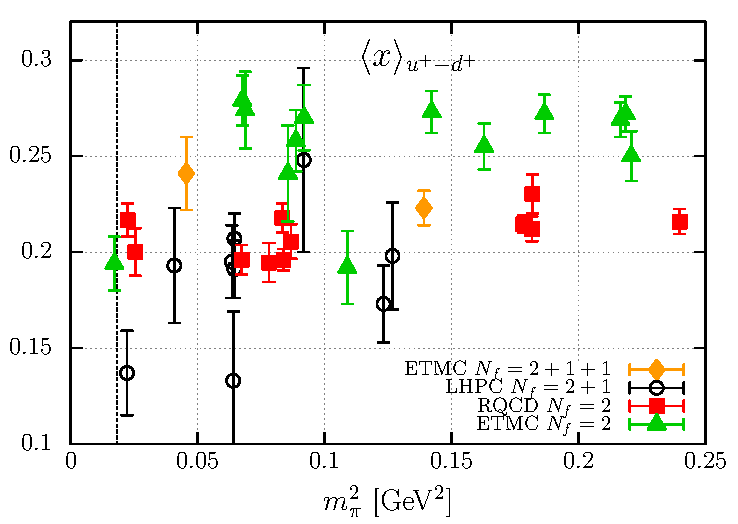
\includegraphics[width=0.49\textwidth]{plots/x_world.pdf}}
\subfloat[]{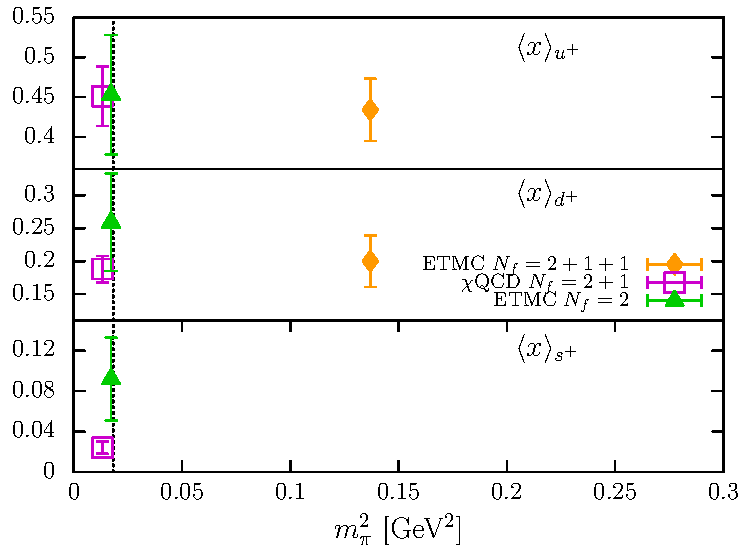
\includegraphics[width=0.47\textwidth]{plots/xq_world_ud.pdf}}
}
\centerline{
\subfloat[]{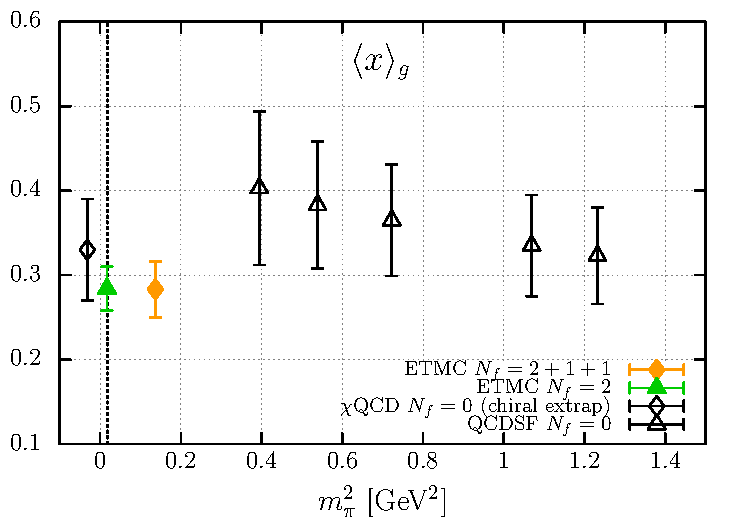
\includegraphics[width=0.49\textwidth]{plots/xg_world.pdf}}
\subfloat[]{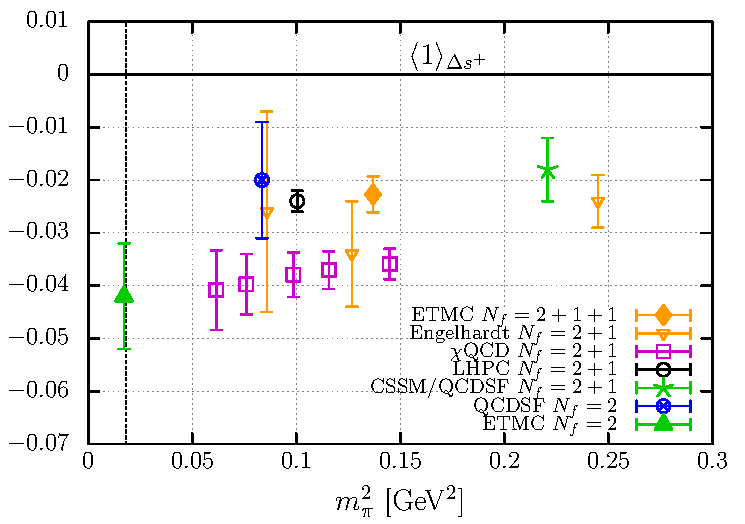
\includegraphics[width=0.49\textwidth]{plots/ga_world_strange.pdf}}
}
\centerline{
\subfloat[]{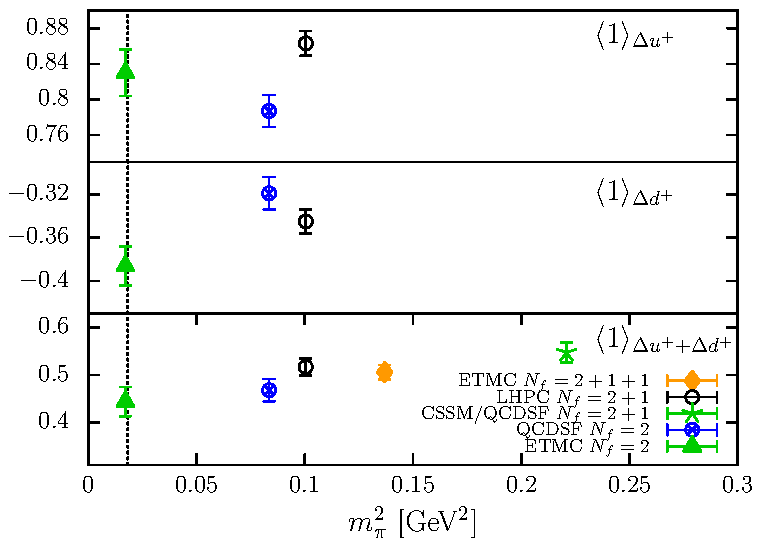
\includegraphics[width=0.47\textwidth]{plots/ga_world_ud.pdf}}
\subfloat[]{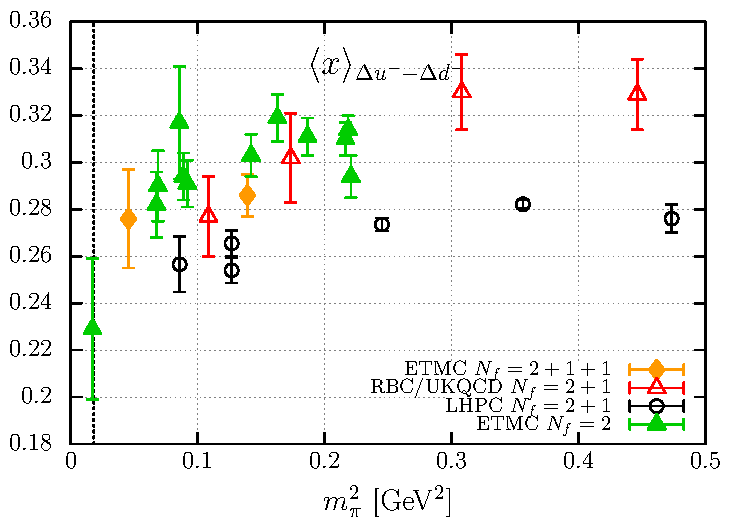
\includegraphics[width=0.49\textwidth]{plots/xdeltaq_isovector.pdf}}
}
\end{center}
\caption{\small Comparison of lattice-QCD results for
  the zeroth and first moments
  of unpolarized and polarized PDFs.
  %
  From left to right and from top to bottom, we show
  results for $\la x\ra_{u^+-d^+}$, $\la x\ra_{q^+}$, $\la x\ra_{g}$,
  $\la 1 \ra_{\Delta s^+}$, $\la 1\ra_{\Delta q^+}$ and
  $\la x\ra_{\Delta u^- - \Delta d^-}$;
  see Tables~\ref{tab:unpolLQCDstatus1B} to~\ref{tab:latticebiblast}
  for details.
}
\label{fig:latt_res}
\end{figure}
%-------------------------------------------------------------------------------






